\section{Qualitative Tracking Results}
\label{sec:blackout}


\begin{figure}[ht!]
\centering
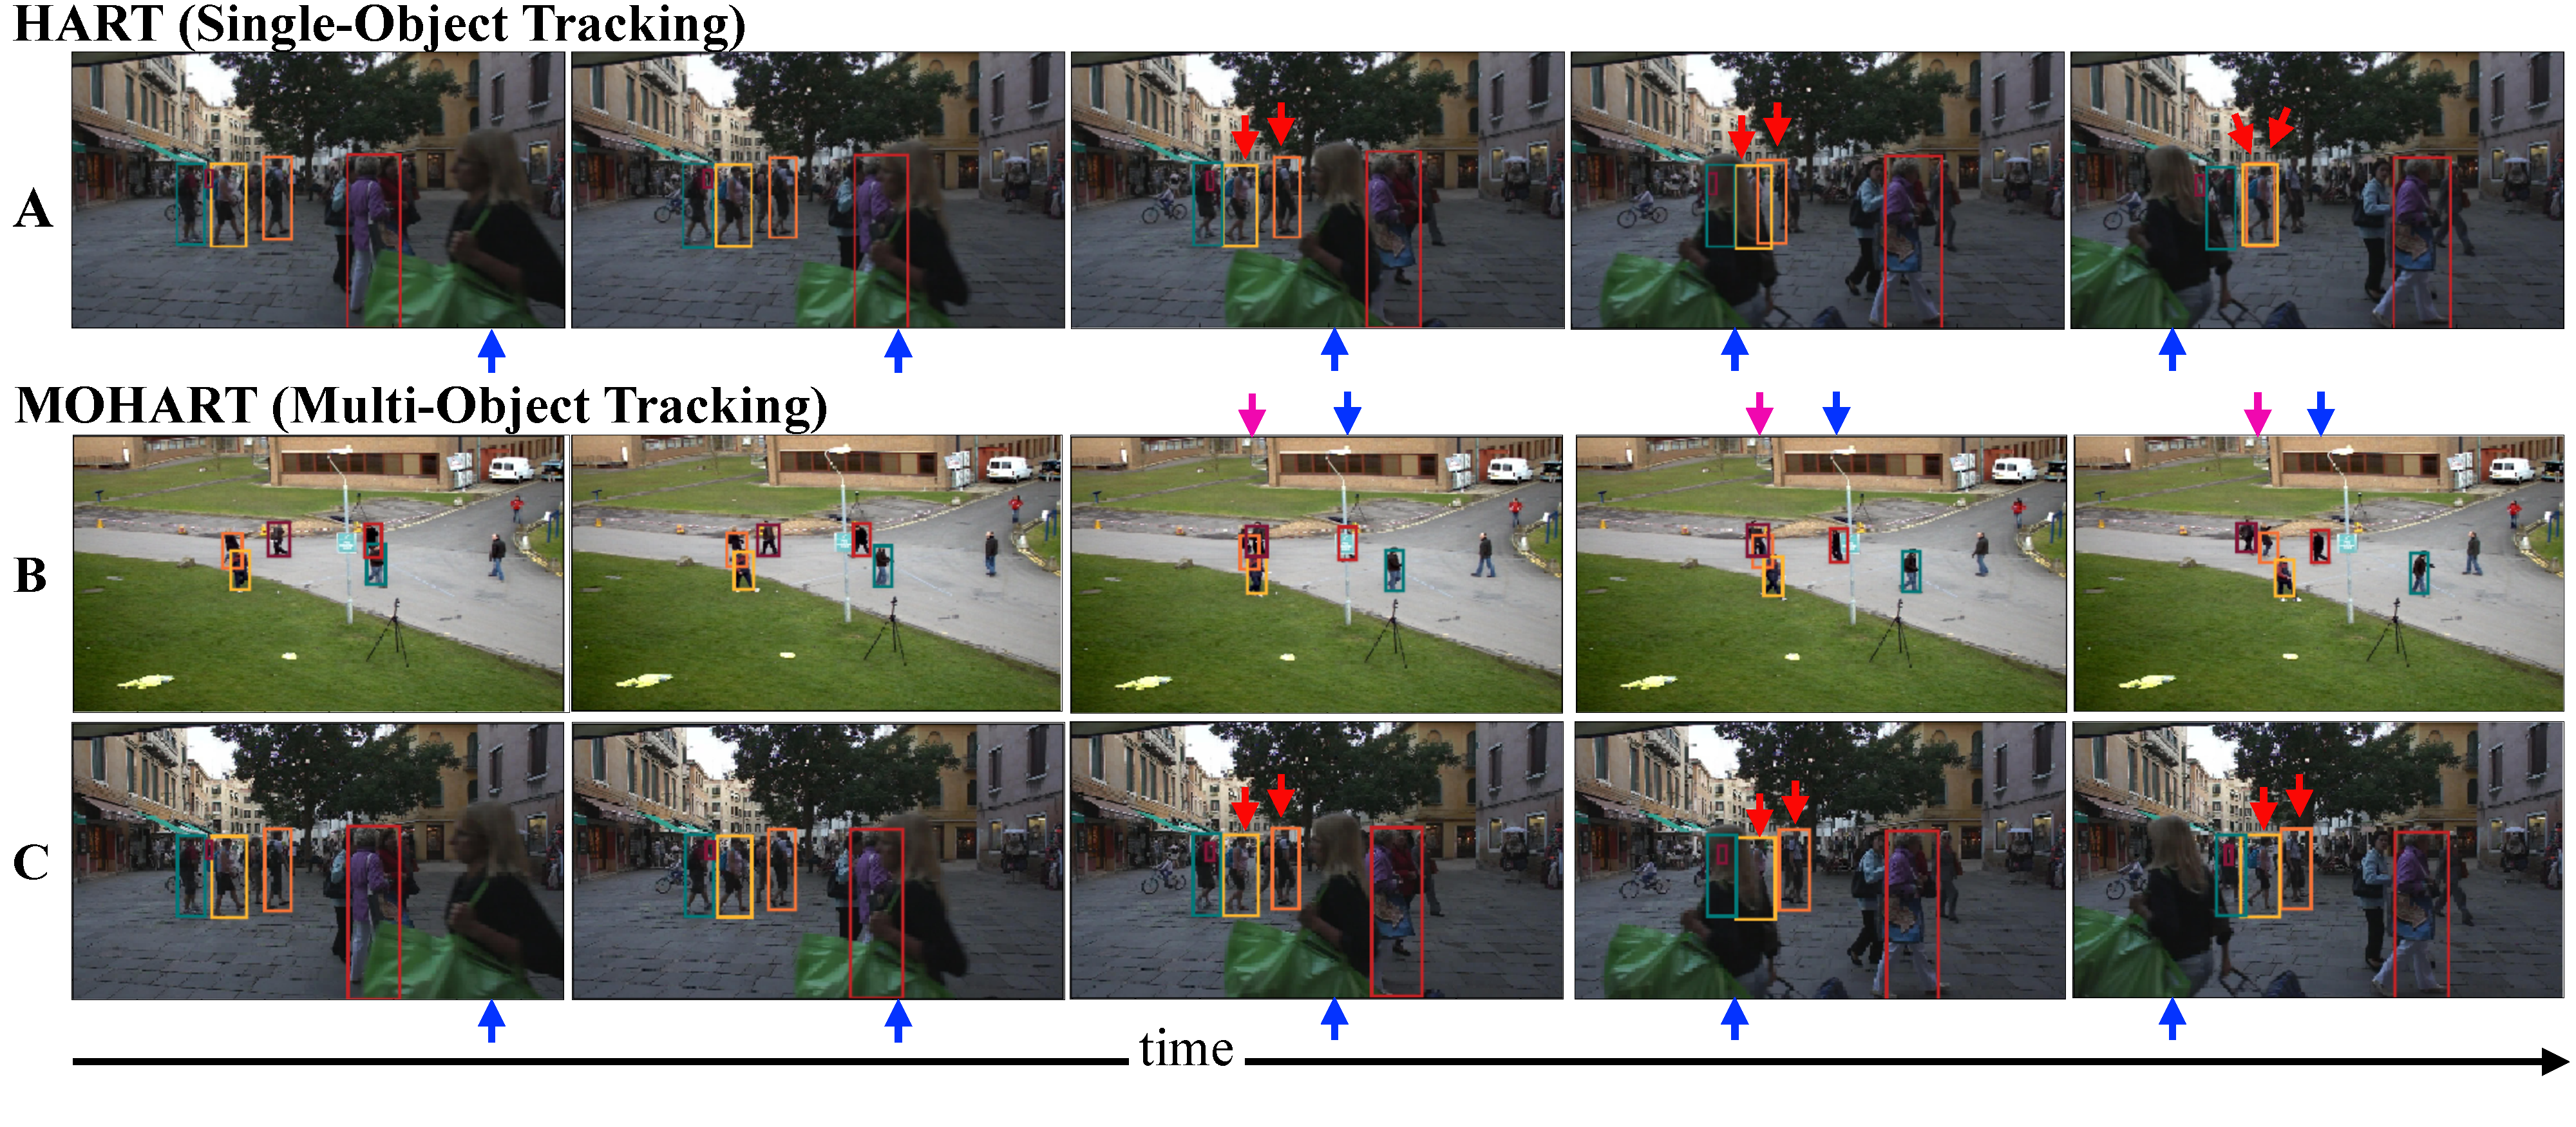
\includegraphics[width=1\textwidth]{figures/MOHART/tracking_qualitative.pdf}
\vspace{-8mm}
\caption{Tracking examples of both \textsc{hart} and \textsc{mohart}. Coloured boxes are bounding boxes predicted by the model, arrows point at challenging aspects of the scenes. (A) \& (C): Each person being tracked is temporarily occluded by a woman walking across the scene (blue arrows). \textsc{mohart}, which includes a relational reasoning module, handles this more robustly (compare red arrows).
\vspace{-4mm}}
\label{fig:tracking_and_predicting}
\end{figure}


%\appendix
\begin{figure}
	\centering
	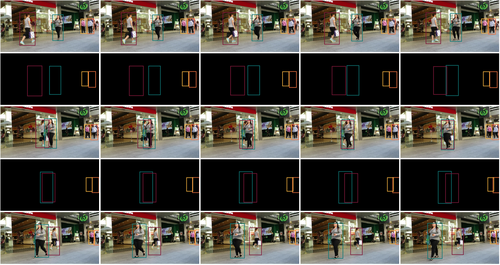
\includegraphics[width=1.0\textwidth]{figures/MOHART/mot_example1.png}
	\vspace{-6mm}
	\caption{Camera blackout experiment on a pedestrian street scene from the MOTChallenge dataset without ego-motion. Subsequent frames are displayed going from top left to bottom right. Shown are the inputs to the model (some of them being black frames, i.e. arrays of zeroes) and bounding boxes predicted by \textsc{MOHART} (coloured boxes). This scene is particularly challenging as occlusion and missing sensor input coincide (fourth row).
		\vspace{-2mm}}
	\label{fig:blackout1}
\end{figure}

% \begin{figure}
% 	\centering
% 	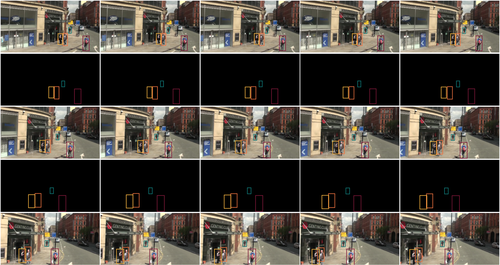
\includegraphics[width=1.0\textwidth]{figures/MOHART/mot_example2.png}
% 	\vspace{-6mm}
% 	\caption{Camera blackout experiment on a street scene from the MOTChallenge dataset with strong ego-motion. The reader is encouraged to compare top left and bottom right frame to make the amount of ego-motion apparent.}
% 	\label{fig:blackout2}
% \end{figure}

In \Cref{sec:experiment_real}, we tested \textsc{mohart} on three different real world data sets and in a number of different setups. \Cref{fig:tracking_and_predicting} shows qualitative results both for \textsc{hart} and \textsc{mohart} on the MOTChallenge dataset.

Furthermore, we conducted a set of camera blackout experiments to test \textsc{mohart}'s capability of dealing with faulty sensor inputs. While traditional pipeline methods require careful consideration of different types of corner cases to properly handle erroneous sensor inputs, \textsc{mohart} is able to capture these automatically, especially when confronted with similar issues in the training scenarios. To simulate this, we replace subsequences of the images with black frames. \Cref{fig:blackout1} and \Cref{fig:blackout_main} show two such examples from the test data together with the model's prediction. \textsc{mohart} learns not to update its internal model when confronted with black frames and instead uses the LSTM to propagate the bounding boxes. When proper sensor input is available again, the model uses this to make a rapid adjustment to its predicted location and `snap' back onto the object. This works remarkably well in both the presence of occlusion (\Cref{fig:blackout1}) and ego-motion (\Cref{fig:blackout_main}). \Cref{tab:results_motc,tab:results_detrac,tab:results_stanford} show that the benefit of relational reasoning is particularly high in these scenarios specifically. These experiments can also be seen as a proof of concept of \textsc{mohart}'s capabalities of predicting future trajectories---and how this profits from relational reasoning.